
In questo capitolo presentiamo la metodologia seguita per il design e la creazione delle applicazioni CAMUS, utilizzando un approccio di visual programming dei mashup. Abbiamo scelto di mettere l'utente finale al centro della nostra progettazione, tenendo conto delle sue esigenze di utilizzo, cercando di mascherare la complessit� delle operazioni. %Esempio Viaggio???%
Nelle sezioni successive saranno esposti i problemi che abbiamo incontrato e le conseguenti scelte progettuali. 
\section{Architettura del sistema\label{sec:architettura-sistema}}

\textcolor{red}{Spiegare com'\`e composta l'architettura (mobile app, server, web app)\\
Scelta di effettuare le query sul server per i servizi primari e sul dispositivo per i servizi di supporto\\
come comunicano le app (flussi e GraphQL)\\
Interazione con l'utente}
L'architettura del sistema CAMUS � composta da tre parti, ognuna delle quali � collegata con l'utente finale del sistema.

\begin{itemize}
	\item \emph{Server.} Il server � l'endpoint al quale si interfaccia l'amministratore del sistema, il quale non ha bisogno di molta astrazione di alto livello per eseguire le sue funzioni. Qui vengono registrati i servizi poi che vengono mappati dall'esperto nel \emph{Visual Design Environment} 
	
	\item \emph{Visual Design Environment.} La piattaforma di visual design ha il compito di costruire le views per i dispositivi mobile e assegnare i termini presenti sul server. 
	
	\item \emph{App Mobile.} 
\end{itemize}

\subsection{Dove eseguire le query verso i servizi?}
%Non sono sicuro di mettere questa sezione qui, poi vediamo dove spostarla
Uno dei primi problemi che abbiamo dovuto affrontare � quello di pensare a come eseguire le richieste verso i servizi esterni. Le due principali soluzioni che vengono adottate nelle piattaforme di mashup per dispositivi mobile sono \emph{Server Mashup} e \emph{Cold Client Mashup} \textcolor{red}{(trovare qualche reference qui?)}
Nel Server Mashup tutte le operazioni vengono eseguite sul server, precisamente, dato un mashup, si occupa di tutte le operazioni di richiesta, integrazione e composizione dei dati, portando tutta la complessit� delle operazioni sul server.
Il Cold Client Mashup, invece, lo schema di mashup viene scaricato sul dispositivo, quindi le operazioni di richiesta, integrazione e composizione vengono eseguite direttamente dal dispositivo.
Entrambe le soluzioni non sono molto bilanciate. Ha senso utilizzare il server come unico componente che esegue tutte le operazioni sui dati e usare l'app mobile solo come semplice browser dove a partire da una richiesta ottengo una o un insieme di risposte? Oppure ha senso spostare tutta la complessit� computazionale sul dispositivo mobile?
Data la crescente potenza di calcolo dei processori destinati al comparto mobile la tentazione di far fare molte operazioni anche complesse al dispositivo mobile � molto forte, tuttavia questo non risolve diverse problematiche.
I servizi non � detto che abbiano i medesimi tempi di risposta, quindi l'applicazione per eseguire una query dovrebbe avere una propria cache. Questo inoltre aggiunge un problema con le API keys dei servizi, che nel caso in cui fossero limitate, porterebbero ad eseguire tante richieste, portando a costi maggiori o a un esaurimento di queries verso il servizio. Questo problema verrebbe risolto utilizzando un unico punto di esecuzione delle query con un meccanismo di caching, in modo da evitare ripetizioni di richieste, tentando di ridurre l'incidenza di questo problema.
Esistono altri due problemi, i quali sono legati all'autonomia e all'utilizzo dei dati del mobile device. L'esecuzione di richieste e operazioni sui dati porta ovviamente a un maggiore consumo di risorse hardware di calcolo e di telecomunicazione, consumando maggiormente la batteria integrata. Con una query unica e con i dati gi� aggregati ovviamente riduce il consumo delle risorse energetiche e dei dati in connessione mobile.

\subsection{Architettura utilizzata}


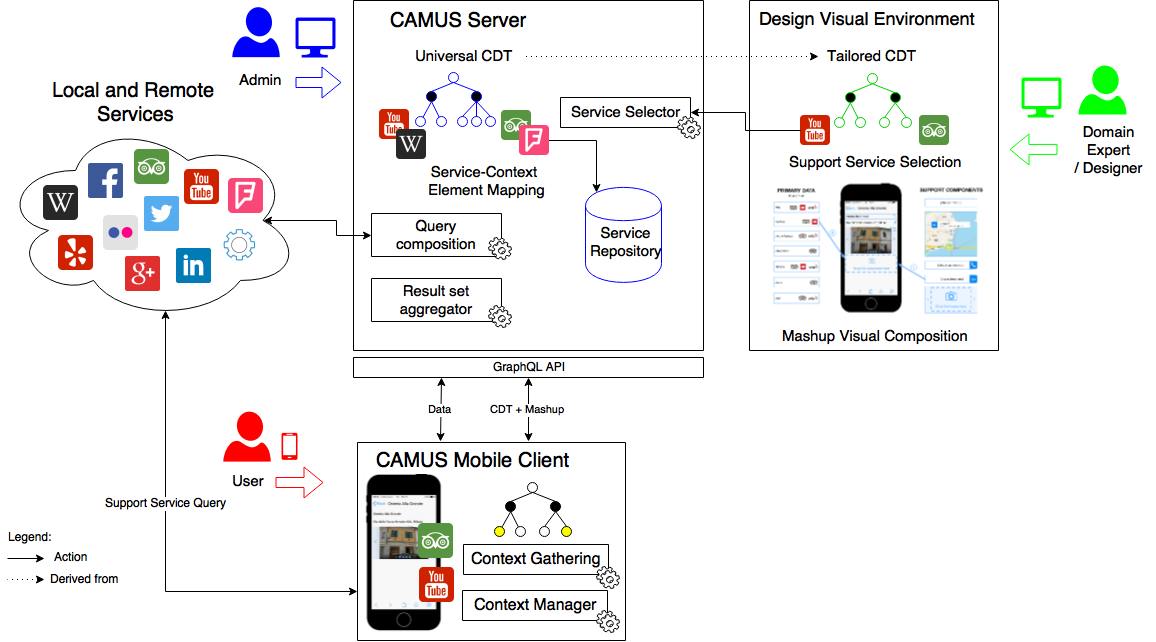
\includegraphics[width=\textwidth]{4-metodologia/Immagini/ArchitectureGen2016.png}

\section{Creazione dell'ecosistema dei servizi\label{sec:ecosistema-servizi}}

I servizi rappresentano un punto cardine del sistema, in quanto mettono a disposizione le risorse che verranno mostrate all'utente. Si � deciso di dividere i servizi in due categorie ben distinte, in base alla funzionalit� del servizio:

\begin{enumerate}
	\item{\emph{Primari}} Sono i servizi che vengono interrogati in prima istanza per acquisire le informazioni relative al contesto nel quale si trova l'utente (es.: Google Places)
	\item{\emph{Supporto}} Sono i servizi che vengono utilizzati per arricchire le informazioni acquisite tramite i servizi primari, come ad esempio le informazioni sul meteo o la cartina geografica del luogo
\end{enumerate}

Per l'acquisizione dei dati � importante che il server sappia come interrogare i servizi e come interpretare le risposte. Si � deciso dunque di creare una repository con tutti i servizi che possono essere utilizzati dal sistema. Questa repository � composta dai \emph{descrittori dei servizi}, che contengono le informazioni necessarie per la gestione dei servizi. I descrittori sono composti dalle seguenti sezioni:

\begin{itemize}
	\item{\emph{Elenco dei parametri}} Per interrogare un servizio � necessario comporre una query con i dati che si vogliono richiedere. Queste informazioni sono dipendenti dalla specifica implementazione del servizio e variano tra un servizio e l'altro. Nel descrittore vengono dunque elencati i parametri necessari per la composizione della query e dove andare a recuperare i relativi valori. L'acquisizione dei valori pu� avvenire secondo tre differenti modalit�:
	\begin{enumerate}
		\item{\emph{Default}} Il valore viene impostato direttamente nel descrittore (es.: l'API key per l'autenticazione)
		\item{\emph{Mapping CDT}} Viene definita l'associazione con uno o pi� nodi del CDT e il valore viene recuperato in base alla selezione effettuata dall'utente (es.: le coordinate geografiche). Questi valori possono essere eventualmente trasformati da quelli simbolici del contesto ad un'altra rappresentazione adatta per effettuare la query (es.: dal valore 'Restaurant' del contesto viene associata la tipologia 'food')
		\item{\emph{Mapping Term}} Questa modalit� viene utilizzata esclusivamente per i servizi di supporto e fornisce un placeholder nelle query che verr� rimpiazzato a runtime con il valore reale acquisito dalla risposta ricevuto o dal dispositivo
	\end{enumerate}
	\item{\emph{Schema della risposta}} Per ottenere omogeneit� tra le risposte ottenute dai diversi servizi, i dati ricevuti devono essere trasformati secondo uno schema comprensibile dalla mobile app. Per effettuare questa trasformazione vengono in aiuto i \emph{termini} (es.: titolo, indirizzo, descrizione, \dots), che rappresentano le classi semantiche di appartenenza degli attributi. L'elenco dei termini disponibili viene mantenuto in una repository come per i descrittori dei servizi. Queste annotazioni hanno una duplice utilit�: in primo luogo, definendo il significato semantico di ogni attributo, semplificano l'integrazione dei dati provenienti da diversi servizi, in secondo luogo semplificano la creazione dei mashup, in quanto permettono di ragionare su categorie astratte di dati rispetto a dati reali forniti dai vari servizi e agevolano la riusabilit� degli schemi in diversi contesti 
	\item{\emph{Gestione della paginazione}} I dati che vengono restituiti a seguito di una query possono essere molteplici. Per semplificare la gestione delle risposte, i servizi implementano delle politiche di paginazione, dove vengono specificati il numero di risultati che si vogliono ottenere in una pagina e un numero che indica la pagina che � stata richiesta \cite{masse2011rest}. Questa sezione serve appositamente per indicare quali sono i parametri che vengono utilizzati dal servizio per richiamare le diverse pagine che compongono i risultati
\end{itemize}

\section{Universal CDT\label{sec:universal-cdt}}

\textcolor{red}{Spiegare come viene applicato il modello teorico in pratica\\
Divisione dei nodi filter e ranking\\
Divisione tra schema globale e tailored}

\section{Associazione dei servizi al CDT\label{sec:associazione-servizi-cdt}}

\textcolor{red}{Come vengono associati i servizi al contesto + ranking}

\section{Mashup Design\label{sec:mashup-design}}

\textcolor{red}{Spiegare lo schema per la generazione dinamica delle schermate\\
Descrizione web app per la creazione degli schemi}

\section{App Execution\label{sec:app-execution}}

\textcolor{red}{Interazione con l'app: flussi delle comunicazioni con il server (login, getPersonalData, contesto, ...)}